%&latex
\documentclass{article}
\usepackage{amstext}
\usepackage{graphicx}
\usepackage{bm}
\usepackage{amsbsy}
\usepackage{algorithm}
\usepackage{amsmath}
\usepackage{hyperref}
\usepackage{framed}
\usepackage[noend]{algpseudocode}
\usepackage{algorithmicx}
\usepackage[normalem]{ulem}

\begin{document}


%+Title

\title{\textbf{Data Structure And Analysis} \\(CSC263)\\Lecture Notes}
\author{Tianquan Di}
\date{\today}
\maketitle
%-Title
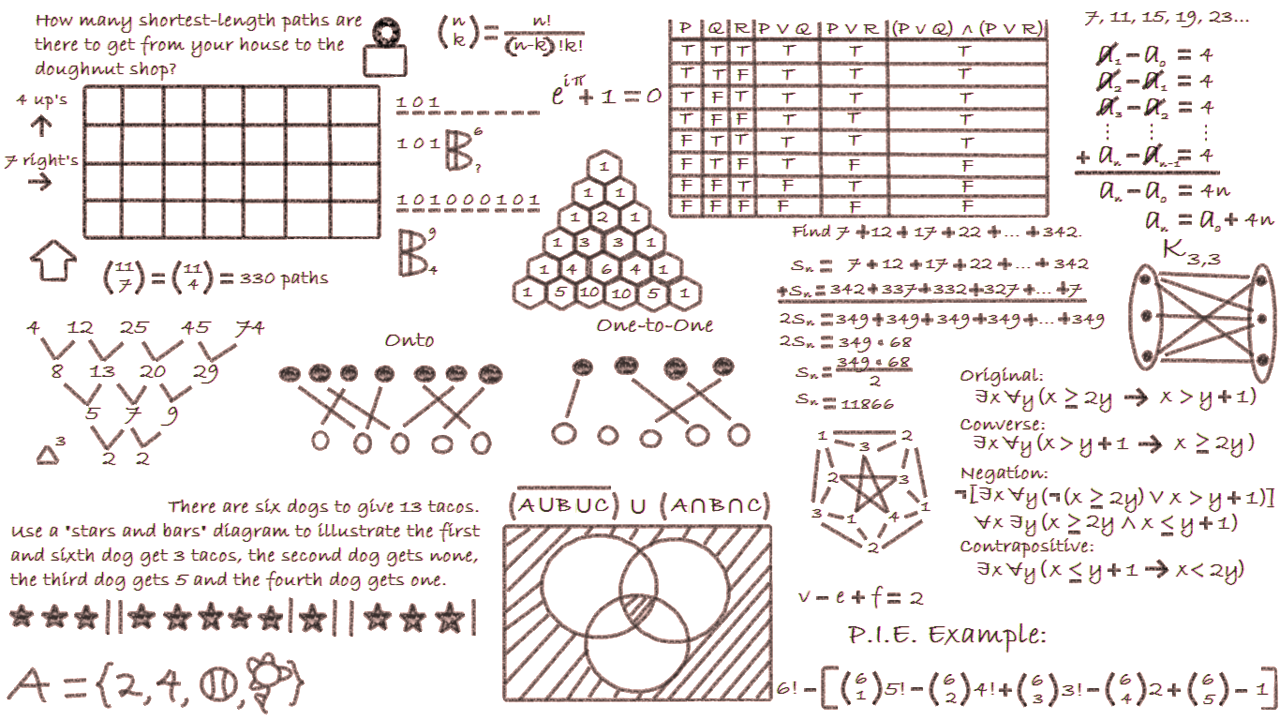
\includegraphics{image003.png}

\newpage
%+Abstract
\begin{abstract}
    \textbf{Why do we need to learn data structures? }This course helps you to explore a new perspective on the algorithm analysis, in the field of Computer Science. CSC263 will also provide you the foundation of technical interviews from your dream tech companies, such as Microsoft, Google, etc. This lecture notes will primarily follow Prof. Sam Toueg's lecture, Prof. David Liu's lecture notes, as well as CLRS. According to Prof. Sam Toueg's description of the course: \quote{Data structures are ways of organizing the data involved in computation, suitable for representation in and manipulation by computers. Algorithms are precisely stated, general problem solving methods. Data structures and algorithms are central to computer science. They are also integrally related: neither can be studied fruitfully without knowledge of the other. This course has two goals: First, to learn several important data structures and algorithms, including how to choose and/or modify a data structure to solve various problems; and second, to introduce the basic tools and techniques for the analysis of algorithms and data structures.}

\begin{center}Course Website: http://www.cs.toronto.edu/~sam/teaching/263/

Textbook: Introduction to Algorithms (i.e. CLRS)

This document assumes that you have the knowledge provided from CSC165 and CSC236.
\end{center}


\end{abstract}
%-Abstract

\newpage
%+Contents
\tableofcontents
%-Contents

\newpage
\section{Review of Growth of Functions}
\subsection{Asymptotic bounds on worst-case time complexity}
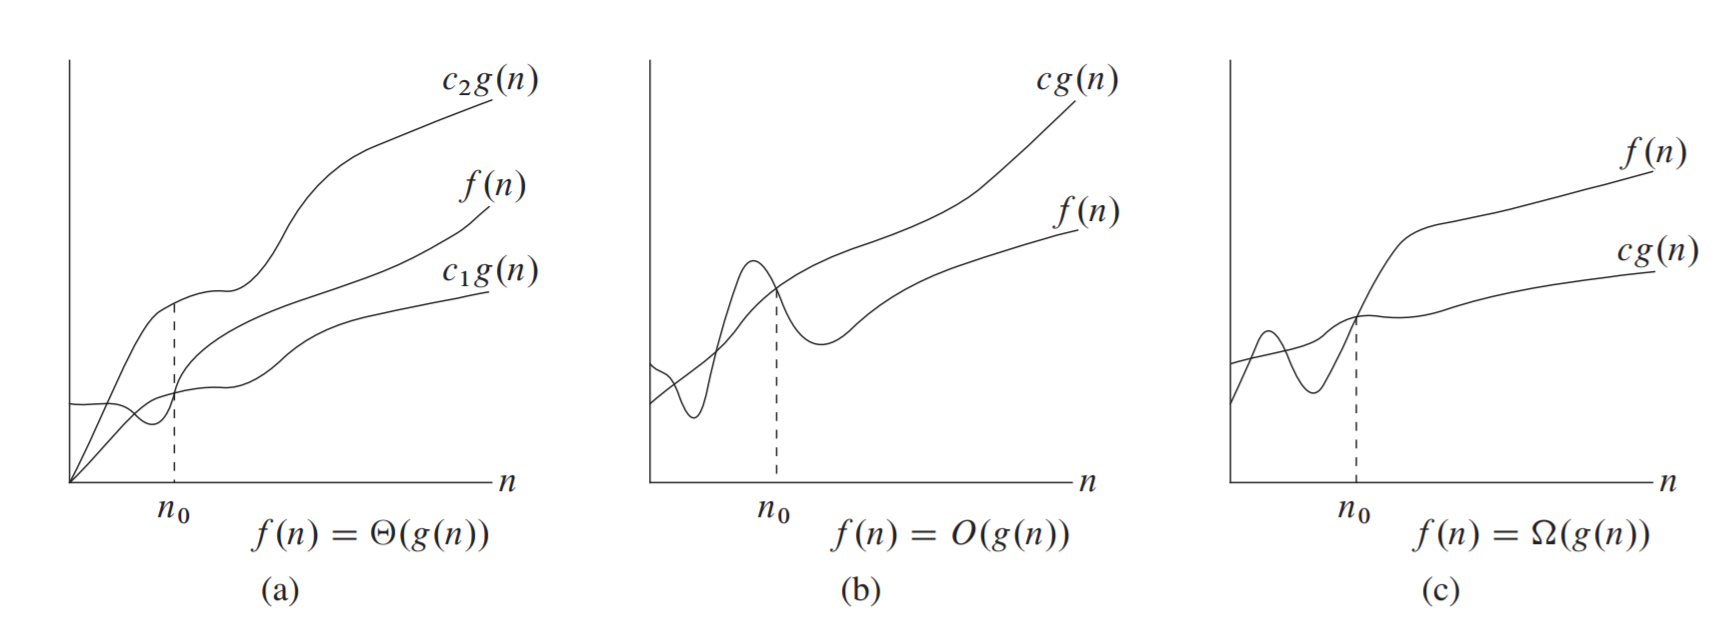
\includegraphics{image001.png}
Let $t(x)$ be the number of steps taken by algorithm $\mathcal{A}$ on the input $x$.\\
Let $T(n)$ be the $worst-case$ time complexity of algorithm $\mathcal{A}$.
Then:
\begin{center}$T(n) = \max_{\textbf{all inputs $x$ of size $n$}} t(x) = \max\{t(x) : x \text{ is an input of size }n\}$\end{center}
\paragraph{To prove that $T(n)$ is $O(g(n))$:} we must show that:\\
$$\exists c >\ 0, \exists n_0 > 0, \forall n > n_0 : T(n) \leq c \cdot g(n)$$
The above statement is equivalent to: \\
$\Leftrightarrow$ max \{$t(x) : $ $x$ is an input of size $n$\} $\leq$ $c \cdot g(n)$ 
\\
$\Leftrightarrow$ For \textbf{every} input $x$ of size $n$, $t(x) \leq c \cdot g(n)$
\\
$\Leftrightarrow$ For \textbf{every} input of size $n$, $\mathcal{A}$ takes \textit{\textbf{at most}} $c \cdot g(n)$ steps.
\paragraph{To prove that $T(n)$ is $\Omega(g(n))$:} we must show that: 
$$\exists c >\ 0, \exists n_0 > 0, \forall n > n_0 : T(n) \geq c \cdot g(n)$$
The above statement is equivalent to: \\
$\Leftrightarrow$ max \{$t(x) : $ $x$ is an input of size $n$\} $\geq$ $c \cdot g(n)$ 
\\
$\Leftrightarrow$ For \textbf{some} input $x$ of size $n$, $t(x) \geq c \cdot g(n)$
\\
$\Leftrightarrow$ For \textbf{some} input of size $n$, $\mathcal{A}$ takes \textit{\textbf{at least}} $c \cdot g(n)$ steps.
\paragraph{To prove that $T(n)$ is $\Theta(g(n))$:} we must show that:
$$\text{$T(n)$ is $O(g(n))$ \textbf{and} $T(n)$ is $\Omega{(g(n))}$}$$
For example, the worst-case time complexity for bubble sort is $\Theta(n^2)$. This means that bubble sort is both $O(n^2)$ and $\Omega(n^2)$. Since bubble sort is $O(n^2)$, for \textbf{every} input of size n, the algorithm takes\textit{ \textbf{at most}} $c_1 \cdot n^2$ steps. Since bubble sort is $\Theta(n^2)$, this means that for \textbf{some} in put of size n, the algorithm takes \textbf{\textit{at least}} $c_2 \cdot n^2$ steps.
\section{Priority Queues \& Heaps}
\subsection{Abstract Data Type (ADT) vs. Data Structure}
Before we start talking about any else, let us discuss about the definition of \textbf{abstract data type} and \textbf{data structure}.\begin{quotation} \noindent An \textbf{abstract data type (ADT)} is a theoretical model of an entity and the set of operations that can be performed on that entity. In other words, it {describes an object and its operations.}\\ \noindent A \textbf{data structure} is {some specific implementation of Abstract Data Type.}\end{quotation}\\
\subsection{The Priority Queue ADT}
Consider the following example, which is the definition for the Priority Quete ADT.
\begin{framed}
\textbf{The Priority Queue ADT}\\
\indent Object: Set S of elements with ``keys'' (priority) that can be compared
\\
\indent Operations: \\
\indent \indent \textbullet \indent \textbf{Insert(S, x): }Insert element x into S.
\\
\indent \indent \textbullet \indent \textbf{Max(S): } Returns the element with the highest priority (i.e. largest key) in S.
\\
\indent \indent \textbullet \indent \textbf{Extract\_Max(S, x): } Returns Max(S) and removes it from S.
\end{framed}
A classic example of priority queues in practice is a hospital waiting
room: more severe injuries and illnesses are generally treated before minor
ones, regardless of when the patients arrived at the hospital.\footnote{Liu, n.d., 23}
\subsection{Heaps}
\begin{flushleft}Our goal is to do all the operations above in $\Theta(log(n))$ time. The solution is to use a \textbf{data structure} called \textbf{Max-Heap}. \end{flushleft}
\begin{table}[h]
\begin{tabular}{|l|l|l|}
\hline
Worst Case Time For   & Insert & Extract\_Max \\ \hline
Unordered Linked List & $\Theta(1)$      &  $\Theta(n)$            \\ \hline
Ordered Linked List   &  $\Theta(n)$      &  $\Theta(1)$            \\ \hline
\textbf{Max Heap}     &  $\Theta(log(n))$ & $\Theta(log(n))$       \\ \hline
\end{tabular}
\end{table}
Before introducing the max-heap, let us talk about the complete binary tree. Definition of a complete binary tree \textbf{complete binary tree (CBT)} is a binary tree such that, for every level $L$ (except the bottom level), the binary tree has $2^L$ nodes. Also, all the nodes at the bottom level are as far left as possible.
\newpage
\begin{figure}
\begin{center}  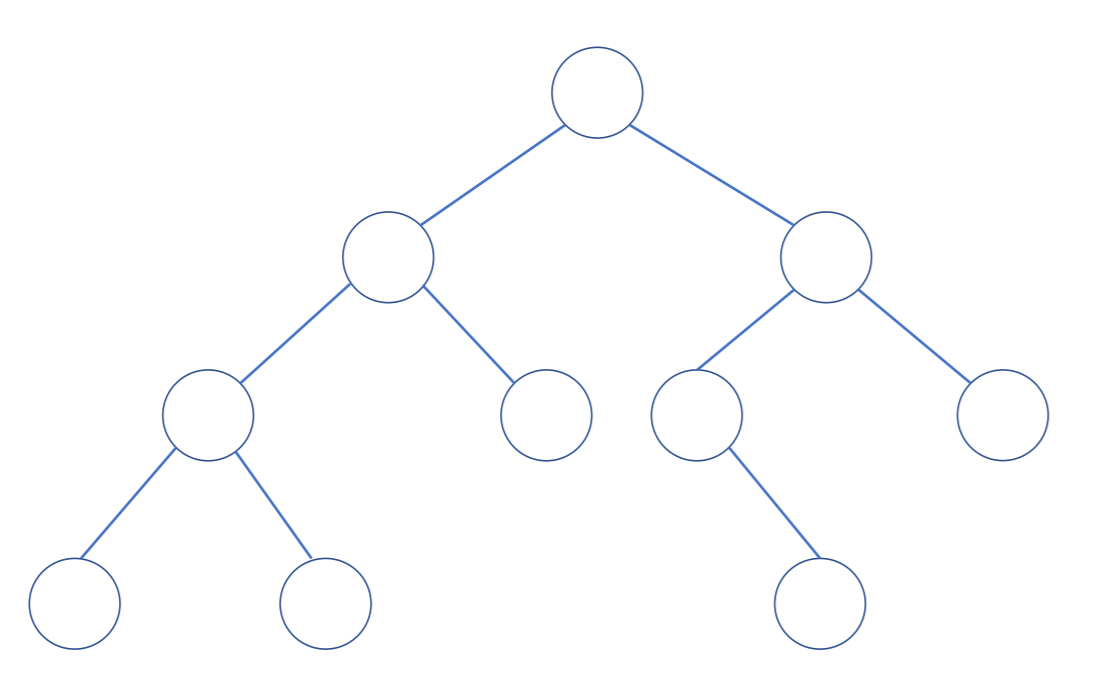
\includegraphics[scale=0.5]{image004.png}\end{center}
  \caption{An example of \textbf{non-complete} binary tree}
  \begin{center}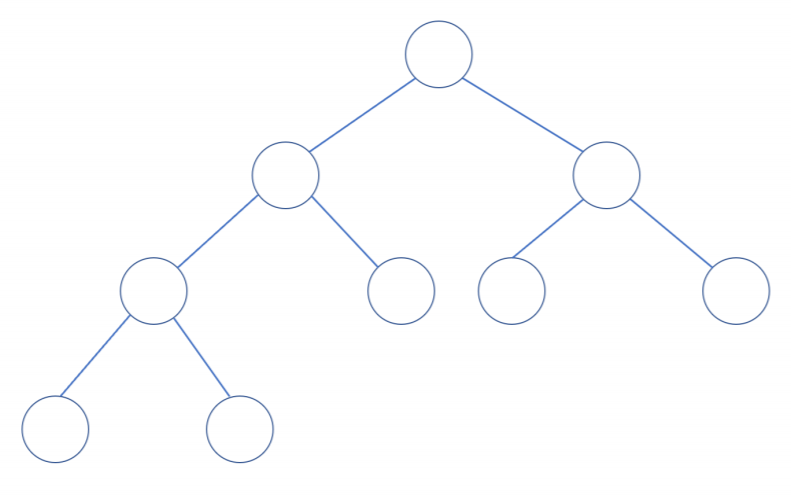
\includegraphics[scale=0.75]{image005.png}\end{center}
  \caption{An example of \textbf{complete} binary tree}
 \end{figure}
\begin{center}\fbox{Fact: Height of a CBT with n nodes is $\lfloor log_2(n)\rfloor$}
\end{center}
A \textbf{max-heap} is a complete binary tree that satisfies \textbf{max-heap property}, which is that the value in each internal node is greater than or equal to the values in the children of that node.
We typically use an \textbf{array} to store a max-heap into the memory.
\begin{figure}[h]\begin{center}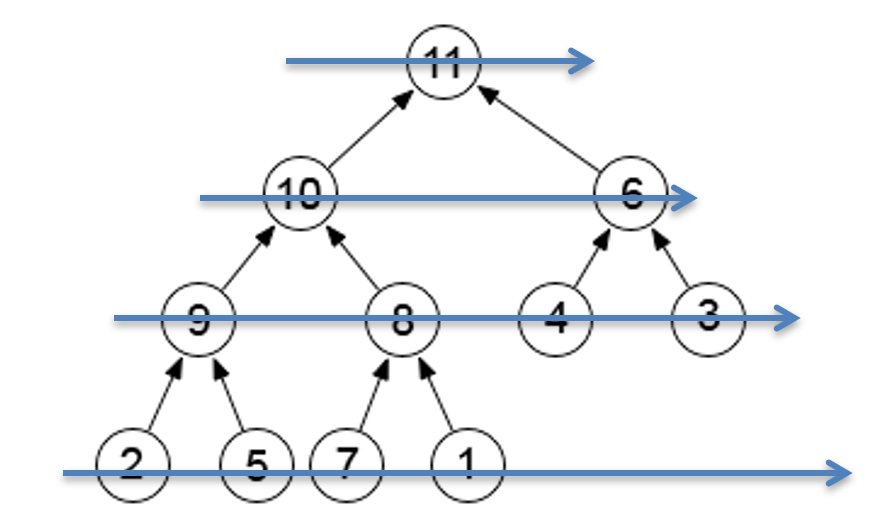
\includegraphics[scale=0.55]{image006.png}\end{center}\caption{The order of elements in an array implementation of a max-heap.}
\end{figure}
\\
Notice from the figure that the array is just the \textbf{level-order traversal} of the max-heap, from \textbf{top \textbf{to bottom}}.
\begin{figure}[h]\begin{center}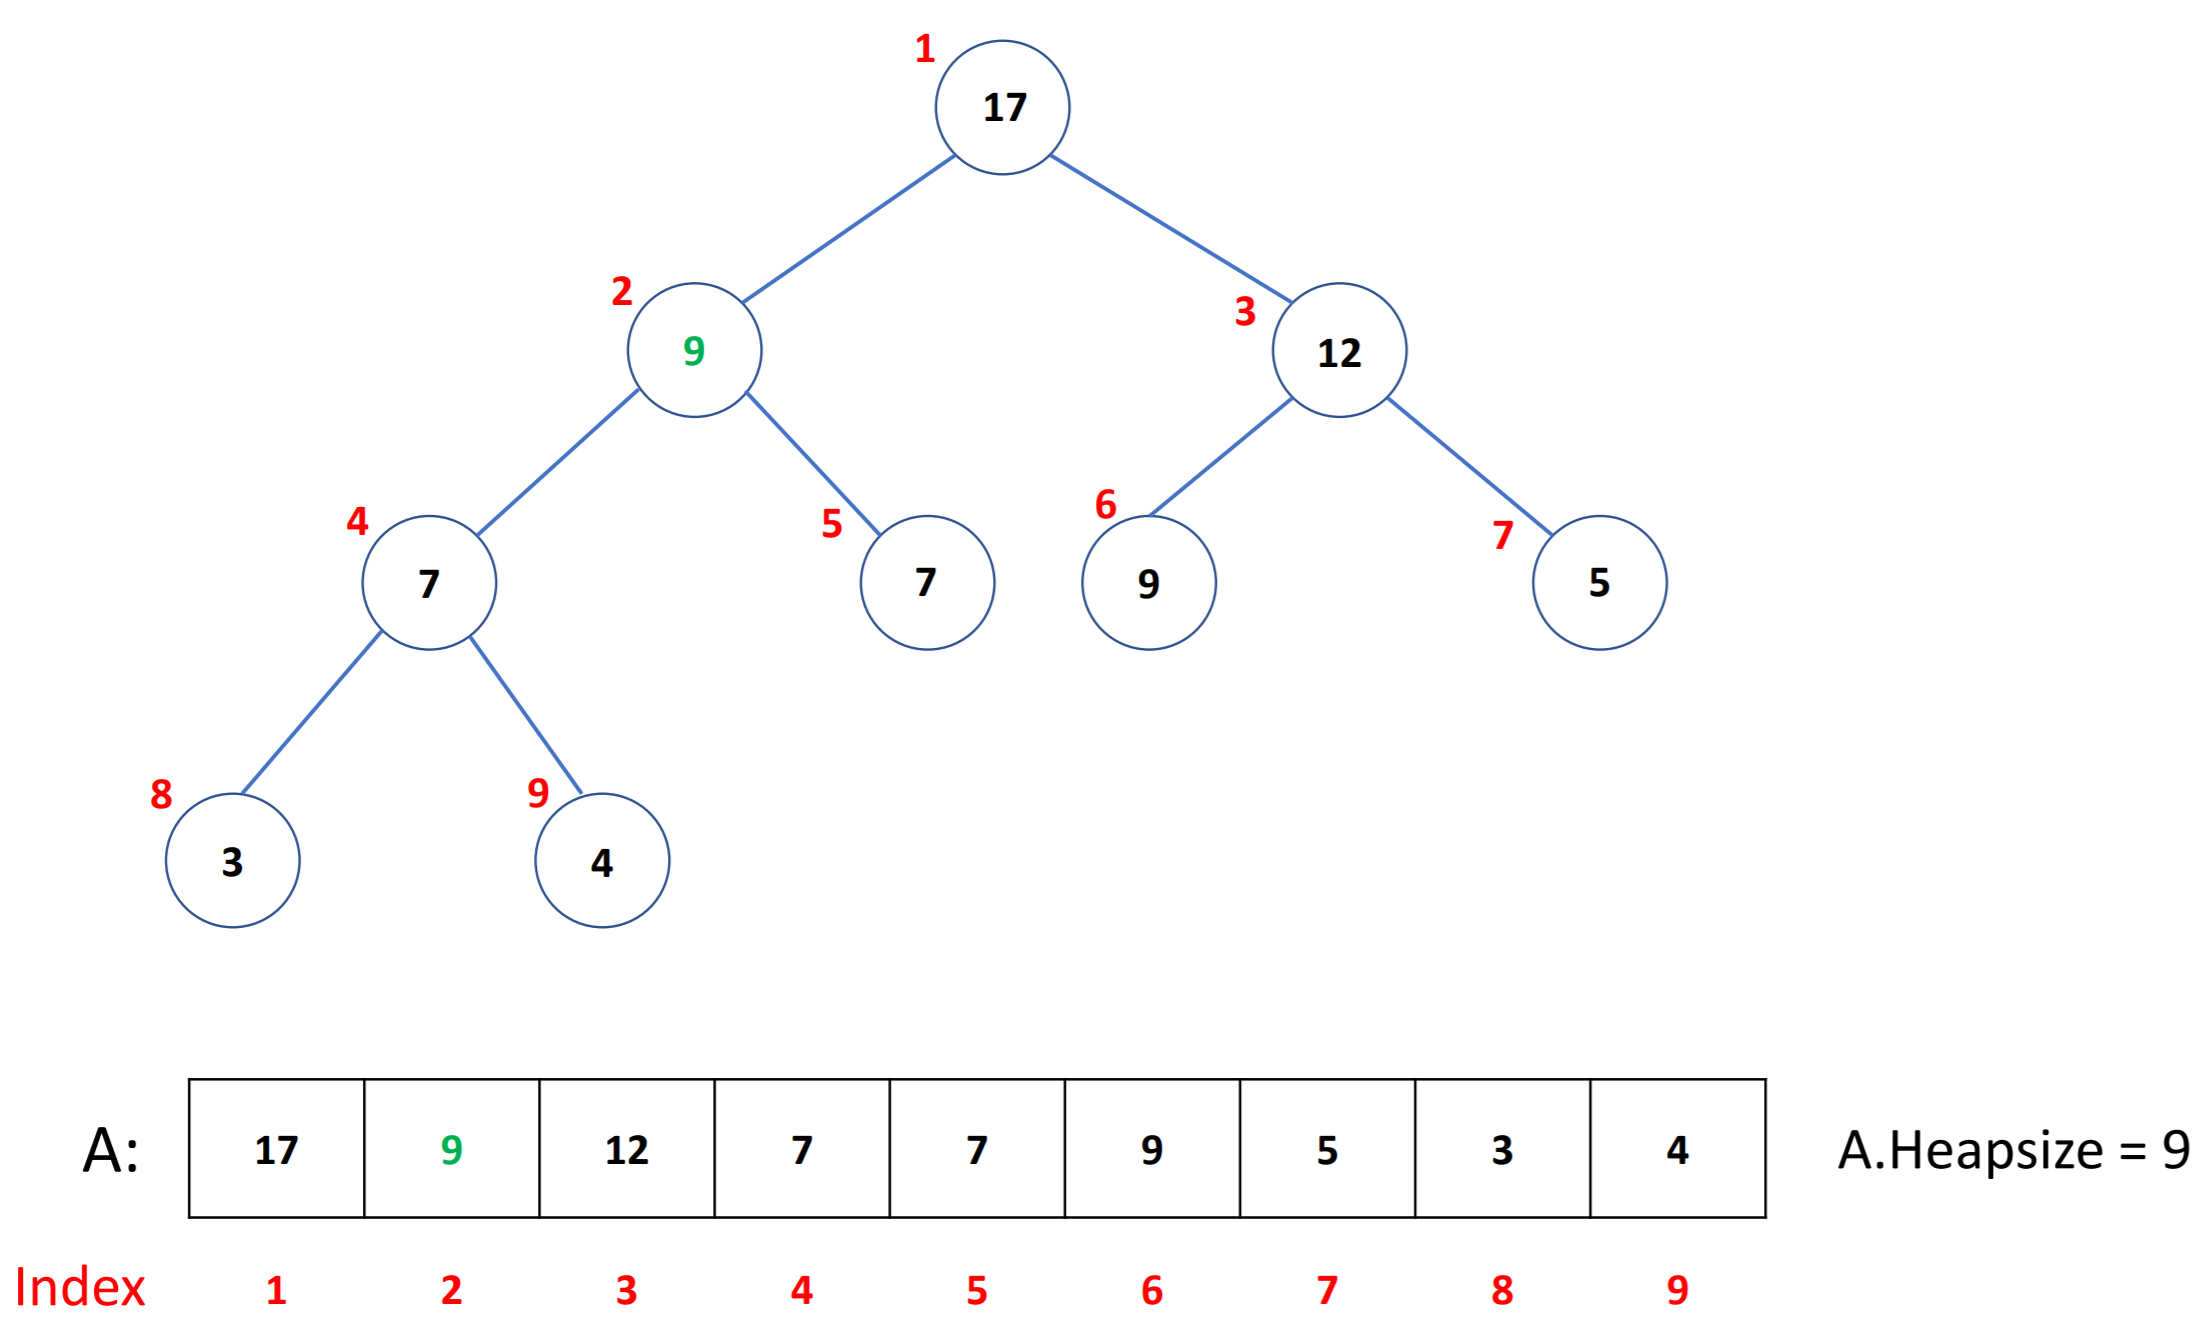
\includegraphics[scale=0.6]{image007.png}\end{center}\caption{A typical example of array representation of a Max-Heap.}\end{figure}
Now let us introduce the operations for the max-heap. \\
\begin{framed}
\textbf{High level idea for operations on Max-Heap}\\
\indent \textbullet  \indent Maintain the Complete Binary Tree shape.\\
\indent \textbullet \indent Maintain the Max-Heap property. 
\end{framed}
\\
\textbf{Insert(S, x): }Insert places a key in a new node that is the last node in a level-order-traversal of the heap. The inserted key is then “``bubbled'' upwards until the heap property is satisfied.
\begin{algorithm}
\caption{The algorithm for insert operation of max-heap.}\label{euclid}
\begin{algorithmic}
\Procedure{Insert}{$A, x$}
\State Put $x$ at the bottom left of the tree:
\State Increment A.heapsize and and set A[A.heapsize] = $x$
\State Bubble $x$ up to the top of the tree:
\While{$x$ is not root \textbf{AND} priority of $x > $ priority of its parent}
\State Swap $x$ with its parent
\end{algorithmic}
\end{algorithm}
\\
Putting $x$ at the bottom left of the tree \textbf{maintains Complete Binary Tree shape}, and bubbling $x$ up to the top of the tree \textbf{maintains the Max-Heap property.} Since the max-heap is a CBT with height $\lfloor log_2(n)\rfloor$, bubbling $x$ up the tree takes is $O(log(n))$. Thus, the worst case running time of the algorithm is $O(log(n))$.\\
\textbf{Max(S)}: We simply get the root of the tree. Thus, the Max algorithm is constant runtime. \\
\textbf{Extract\_Max(S, x): }
\begin{algorithm}
\caption{The algorithm for extract-max operation of max-heap.}\label{euclid}
\begin{algorithmic}
\Procedure{Extract\_Max}{$A, x$}
\State Return the root A[1].
\State Remove the returned element from the heap: 
\State \indent Set A[1] = A[A.heapsize] and decrement A.heapsize
\State Drip the element in A[1] down the tree:
\State \indent Let $x$ be the element in A[1]\While{$x$ is not a leaf \textbf{AND} priority of some child of $x > $priority of $x$}
\State Swap $x$ with the highest-priority of child of $x$
\end{algorithmic}
\end{algorithm}
\subsection{Mergeable Priority Queue ADT and Binomial Heaps}
\begin{table}[h]
\begin{tabular}{|l|l|l|l|l|l|}
\hline
Abstract Data Types      & Data Structures   & Insert & Min & Extract\_Min & Union \\ \hline
Priority Queues          & Min Heap          &    Yes    &  Yes   & Yes             &   \textbf{No}    \\ \hline
\textbf{Mergable} Priority Queues & Min \textbf{Binomial} Heaps &   Yes     &   Yes  & Yes             &   \textbf{Yes}    \\ \hline
\end{tabular}
\end{table}
\\
Elements of binomial heaps are stored in a \textbf{sequence} of \textbf{binomial trees}. (i.e. Binomial Forests)
\begin{figure}[h]
\begin{center}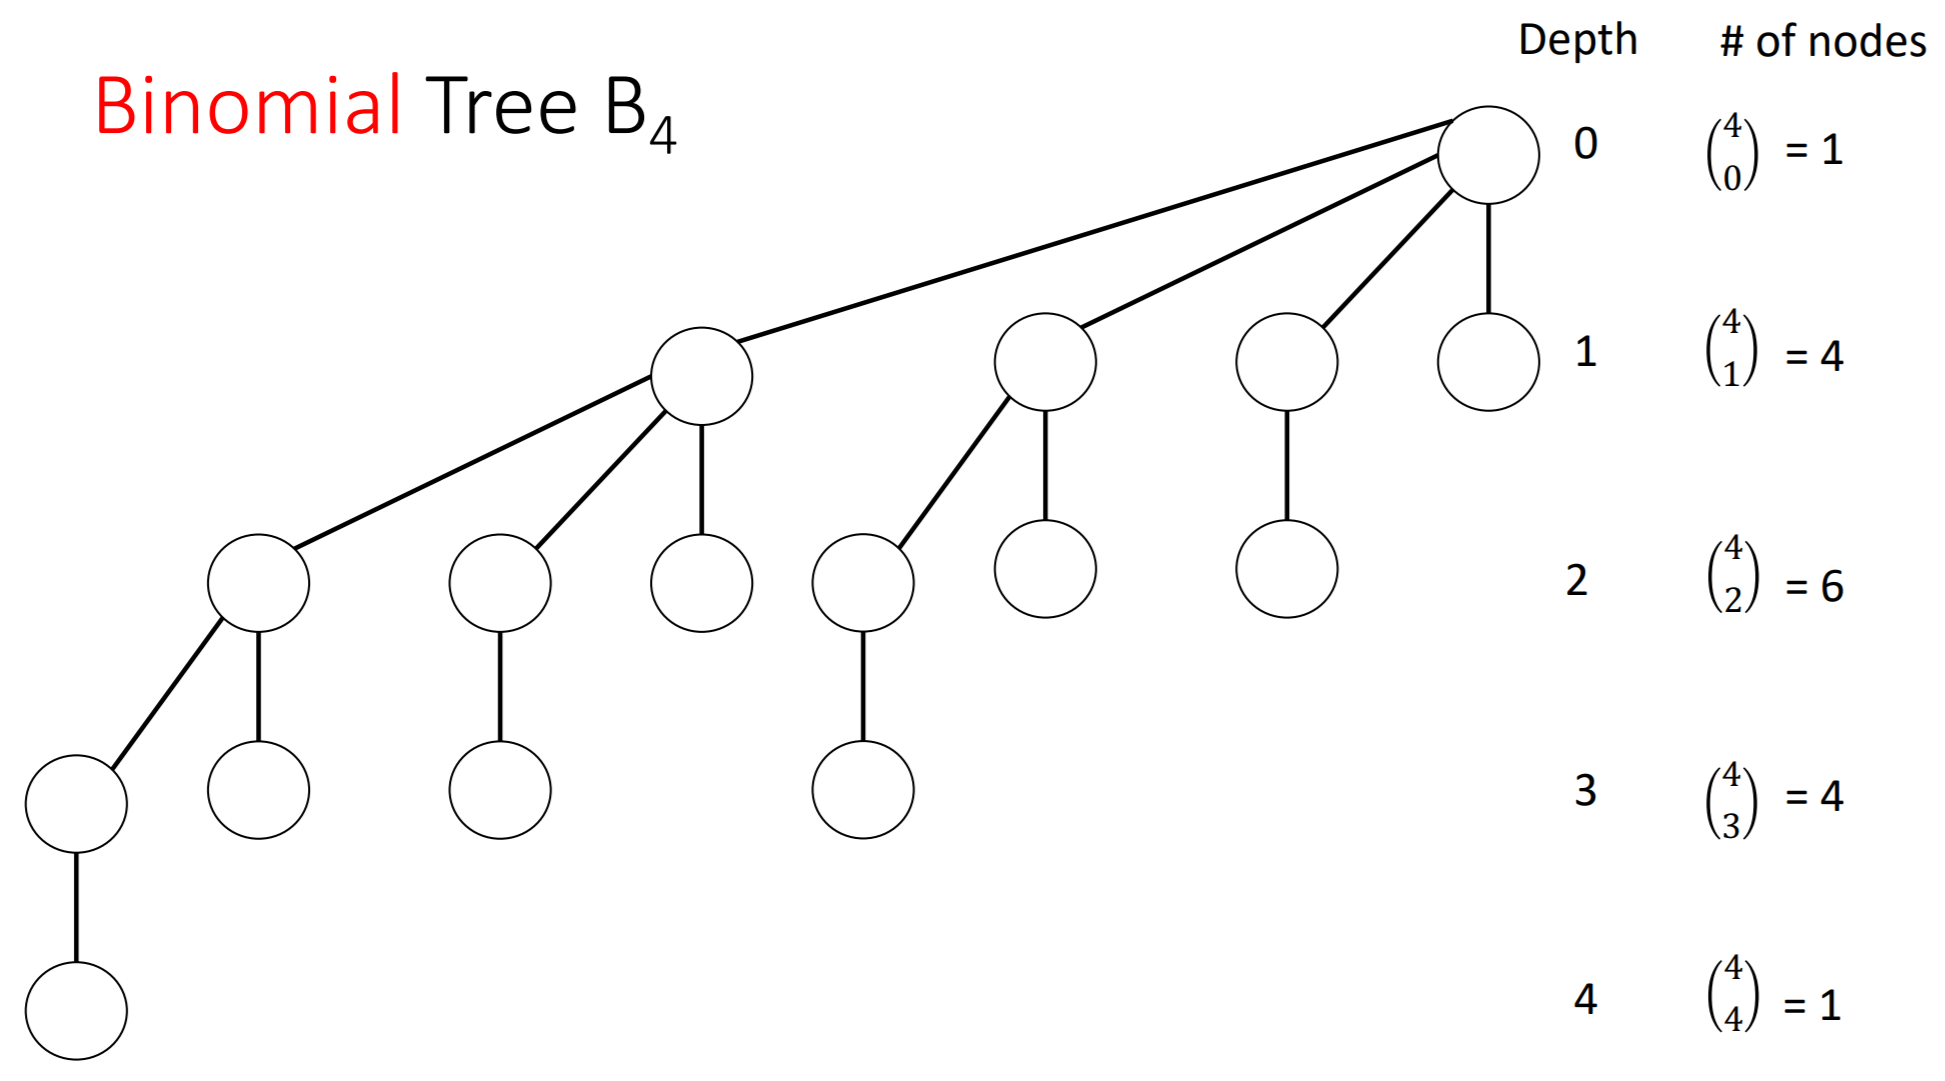
\includegraphics[scale=0.7]{image008.png}\end{center}
\caption{A visualization of binomial tree,  $B_4$.}
\end{figure}

\begin{figure}[h]
\begin{center}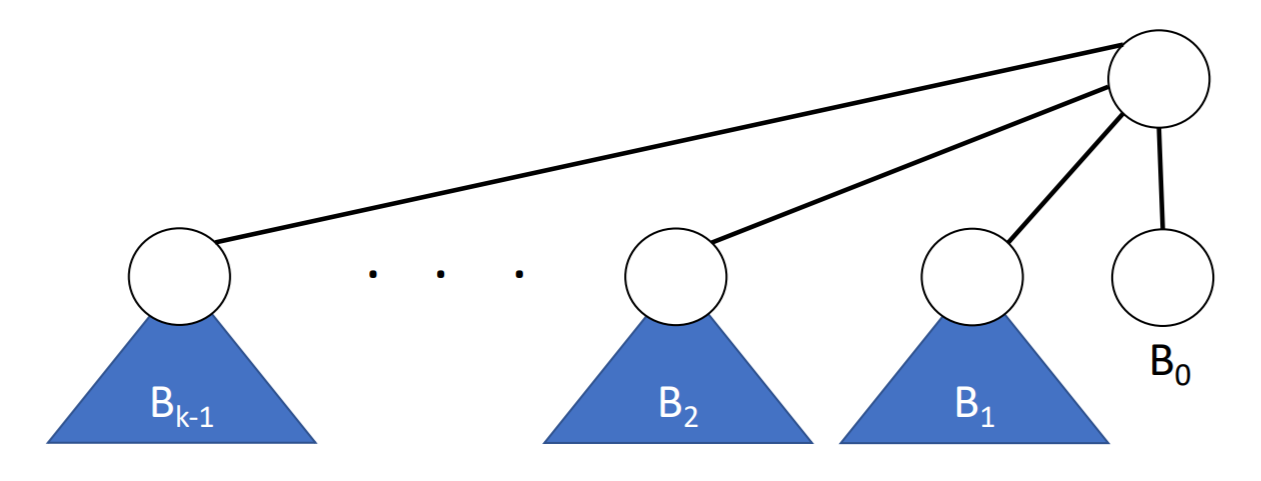
\includegraphics[scale=0.8]{image009.png}\end{center}
\caption{A more general visualization of binomial tree,  $B_k$.}
\end{figure}
\\
\begin{framed}
\textbf{Properties of Binomial Tree, $B_k$: }
\begin{itemize}
  \item Height $k$
  \item $2^k$ nodes
  \item $\binom{k}{d}$ nodes at depth $d$
\end{itemize}
\end{framed}
A \textbf{Binomial Forest} is a sequence of $B_k$ trees with strictly decreasing k’'s and a total of n nodes.
\begin{framed}
\textbf{Binomial Forest $F_n$: }
\begin{itemize}
\item $F_n$ has $n$ nodes.
\item $n =\  <b_t,b_{t-1},...,b_0>_2.$ Note that $t = \lfloor log_2(n) \rfloor$
\item $F_n =\ <\text{all trees $B_i$ such that bit $b_i = 1$}>$
\end{itemize}
\end{framed}
\noindent
\subsection{Implementation of operations on Binomial Heaps}
\paragraph{Union(T, Q): }$S \gets Union (T, Q)$: Think about binary addition. Additional info about this to be appeared later.  
\paragraph{To analyze the worst-case time complexity of Union: }
Let $|T| \leq n$ and $|Q| \leq n$ (i.e. each contains at most n elements). This implies that each of T, Q have $O(log(n))$ $B_k$ trees. Then Union(T,Q) takes at most $O(log(n))$ key-comparisions. Hence the worst-case time complexity of the algorithm is $O(log(n))$. 
\paragraph{Insert(T, x): }Simply apply this statement: $S \gets Union (T, x)$

\paragraph{Min(T):} Scan the roots of the $B_k$ trees of $T$ and return the smallest key.
\newpage
\noindent \textbf{Extract\_Min(T)}:
The idea of Extract\_Min can be expressed as follow.\begin{algorithm}[h]
\caption{The algorithm for Extract\_Min for binomial min heap.}\label{euclid}
\begin{algorithmic}
\Procedure{Extract\_Min}{$T$}
\State // Do Min(T) to locate the smallest element
\State $U \gets T - B_i$
\State // Delete root of $B_i$. By lemma 2, we get a binomial heap $S$, where:
\State $S \gets B_i - \text{root of $B_i$}$
\State $T \gets Union(U,S)$
\end{algorithmic}
\end{algorithm}\\
\section{Dictionary (I: AVL Trees}
\subsection{Abstract Data Type: Dictionary}
\paragraph{Object: }Set S of (element with) keys
\paragraph{Operations: }
\begin{itemize}
\item Search(S,x): Returns element with key x, if x is in S; else return ``Not Found''
\item Insert(S,x): Inserts x into S.
\item Delete(S, x): Deletes x from S.
\end{itemize}
\textbf{We want all the operations to be done in log time complexity. That is $\Theta$(log n). Possible solution: Binary Search Tree(BST).}
\subsection{AVL Trees: Intro}
Use BST as the data structure for the dictionary ADT can be slow. For example, if we have a balanced BST and we keep inserting node to the rightmost corner. Then the search would take $\Theta(n)$ time.\paragraph{Balanced BST: }We want BST trees with height $\Theta(log\ n)$. So the operations, including search, insert, delete, will have log time complexity. Solution is to use \textbf{balanced} \textbf{BSTs}. 

\paragraph{AVL Trees: } AVL tree is \textbf{a type} of self-balancing BST. For AVL Trees, the \textbf{balance factor} of each node is always \textbf{between -1 and 1.}
\paragraph{Balance Factor(BF) of a node v in AVL Trees: }\begin{center}{\textbf{BF(v) = height(right subtree of v) - height(left subtree of v)}}\\
\end{center}
\paragraph{Properties of AVL Trees: }
\begin{itemize}
\item AVL trees of n nodes has height $\Theta(log\ n)$; height $\leq 1.44 \ log_2(n+2)$
\item Can do inserts, deletes while maintaining the tree balance in $\Theta(log\ n)$ time.
\end{itemize}
\subsection{AVL Trees: Insert Operation}
\paragraph{General Idea: }
\begin{itemize}
\item Insert x into T as in any BST
\item Go up from x to the root:
\begin{itemize}
\item For each node:
\begin{itemize}
\item 
Adjust the Balance Factor
\item
``Rebalance'' if $BF > 1 \text{ or }BF < -1$
\end{itemize}
\end{itemize}
\end{itemize}
\paragraph{Specific Implementation: }
\begin{itemize}
\item Insert x into T as in any BST:
\begin{itemize}
\item x is now a leaf
\item Set BF(x) to 0 (Since it has no children, balance factor is of course 0.)
\end{itemize}
\item Go up \textbf{from x to the root} and \textbf{for each node v} in this path: 
\begin{itemize}
\item Adjust the BF:
\begin{itemize}b
\item 
if x is in right subtree of v: Increment BF(v)
\item
if x is in left subtree of v: Decrement BF(v)
\item if BF(v) = 0: Stop
\end{itemize}
\item Rebalance if necessary:
\begin{itemize}
\item 
if BF(v) = +2:
\begin{itemize}
\item 
if BF(v.right) = +1: Do \textbf{Left Rotation}, update BFs of rotated nodes, and \textbf{stop.}
\item 
if BF(v.right) = -1: Do \textbf{Right-Left Rotation, }update BFs of rotated nodes, and \textbf{stop}.
\end{itemize}
\item if BF(v) = -2:
\begin{itemize}
\item 
Symmetric to above case.
\end{itemize}
\end{itemize}
\end{itemize}
\end{itemize}
\paragraph{Exercise: How to implement Delete and Search?}
\subsection{Augmentation of AVL Trees}
Coming Soon...
\section{Randomized Algorithms}
You want an algorithm that haves well for \textbf{every possible input.}

\subsection{Randomized QuickSort Algorithm (RQS)}
\paragraph{Input: }Set S of $n$ distinct keys
\paragraph{Output: }Keys of S in increasing order.
\\
It is a recursive divide-and-conquer algorithm.
\paragraph{High-level Description: }
\begin{itemize}
\item If S is empty then return.
\item If $|S| =1$  then output the key in S.
\item Select a key $p$ (``Pivot'') uniformly at random from S:
\begin{itemize}
\item 
By comparing $p$ to every other key in S, split S into:
\begin{itemize}
\item 
$S_< = \{s \in S | s < p \}$
\item
$S_> = \{s \in S | s > p\}$
\end{itemize}
\end{itemize}
\item $RQS(S_<)$; output $p$; $RQS(S_>)$
\end{itemize}
\paragraph{Basic Properties of RQS}

\begin{itemize}
\item Two keys are compared if and only if one of them is selected as a pivot.
\item Two keys are compared at most once.
\item If two keys are ``split apart'' in different sets by a pivot (like 2 and 7 are split apart by pivot 4) then they are never compared.
\end{itemize}

\paragraph{Another Example: } \uline{Fix} an input S. run RQS(S). Let $C =\ $number of key comparisions done by QRS(S). In this case, $C$ is a \textbf{random variable.} Thus, it has an expected value. \textbf{What is the expected value of C, E(C), over all possible random pivot selections done by RQS?}\\
\begin{itemize}
\item 
Let $z_1 < z_2 <...<z_i<...<z_j<...<z_n$, where $i < j$, each $z$ is a key.
\item
Let's say there is a random variable $c_{ij}$. 
$c_{ij} = \begin{cases}
1, \text{iff $z_i$ and $z_j$ are compared by RQS(S)}\\
0, \text{otherwise}\\
\end{cases}
$
\end{itemize}
\begin{align}
C &= \sum_{1 \leq i < j \leq n}c_{ij}\\
E(C) &= E(\sum_{i < j} c_{ij}) = \sum_{i < j} E(c_{ij})\\
E(c_{ij}) &= 1 \cdot P(c_{ij} = 1) + 0 \cdot P(c_{ij} = 0)\\
&= P(c_{ij} = 1)\\
E(c_{ij}) &= P(\text{$z_i$ and $z_j$ are compared by RQS(S)}) = \frac{2}{j - i +1} \text{(Why?)}\\
E(C) &=\sum_{1 \leq i < j \leq n} \frac{2}{j - i + 1} = ... = {2n \cdot (1 + \frac{1}{2} + \frac{1}{3}  + ... +\frac{1}{n})} 
\end{align}

$H_n$ ($H_n$ is denoted as the harmonic series) is O(log n). We have a question remaining:
Why E(cij) equals that? because for two keys to be compared, if only if one of them is selected as a pivot. If we chose anything in between, they can NEVER be compared. So the case must be that we chose one of them as the pivot. Look at the specific example from the slide. Smallest key is 1 and the largest key is 8. 
\end{document}


 


